\section{Results and Static Timing Analysis}
In this final section, we will discuss the results and the performance of our hardware module.
\begin{figure}[!ht]
    \centering
    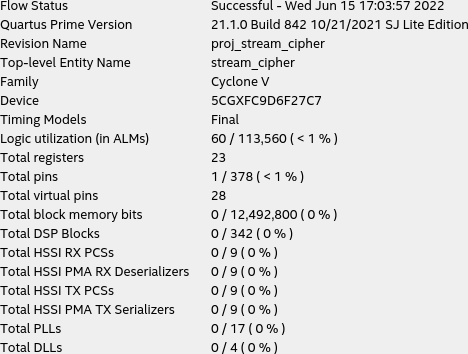
\includegraphics[width=.8\textwidth]{summary}
    \caption{Summary}
    \label{fig:summary}
\end{figure}

The usage of the hardware resources of the target FPGA is very low ($< 1\%$). The number of total used pins is 28, as expected.

Regarding the timing analysis, we have defined a timing constraints file specifying a
target frequency of 100MHz (i.e. 10 nanoseconds clock period). Moreover, for each unconstrained path (input/output signals), we have defined maximum and minimum delay as a percentage of the system clock, 20\% and 10\% respectively. We have reached a frequency of $133.32$MHz at 85°C, and a frequency of $132.89$MHz at 0°C. In both case, the frequency is higher than the predetermined one ($100$MHz), and all constraints are met.